\chapter{Planificación temporal}
\label{chap:planificacion}

La planificación general del proyecto siguiendo un modelo SCRUM, empleando para ello el panel de tareas Trello; un gestor de proyectos que permite aplicar una metodología de desarrollo ágil SCRUM para la realización del mismo.\\

El panel está accesible en el siguiente enlace: \url{https://trello.com/b/SpIbFI7k/robotui}.

\begin{figure}[H]
\hspace*{-.2in}{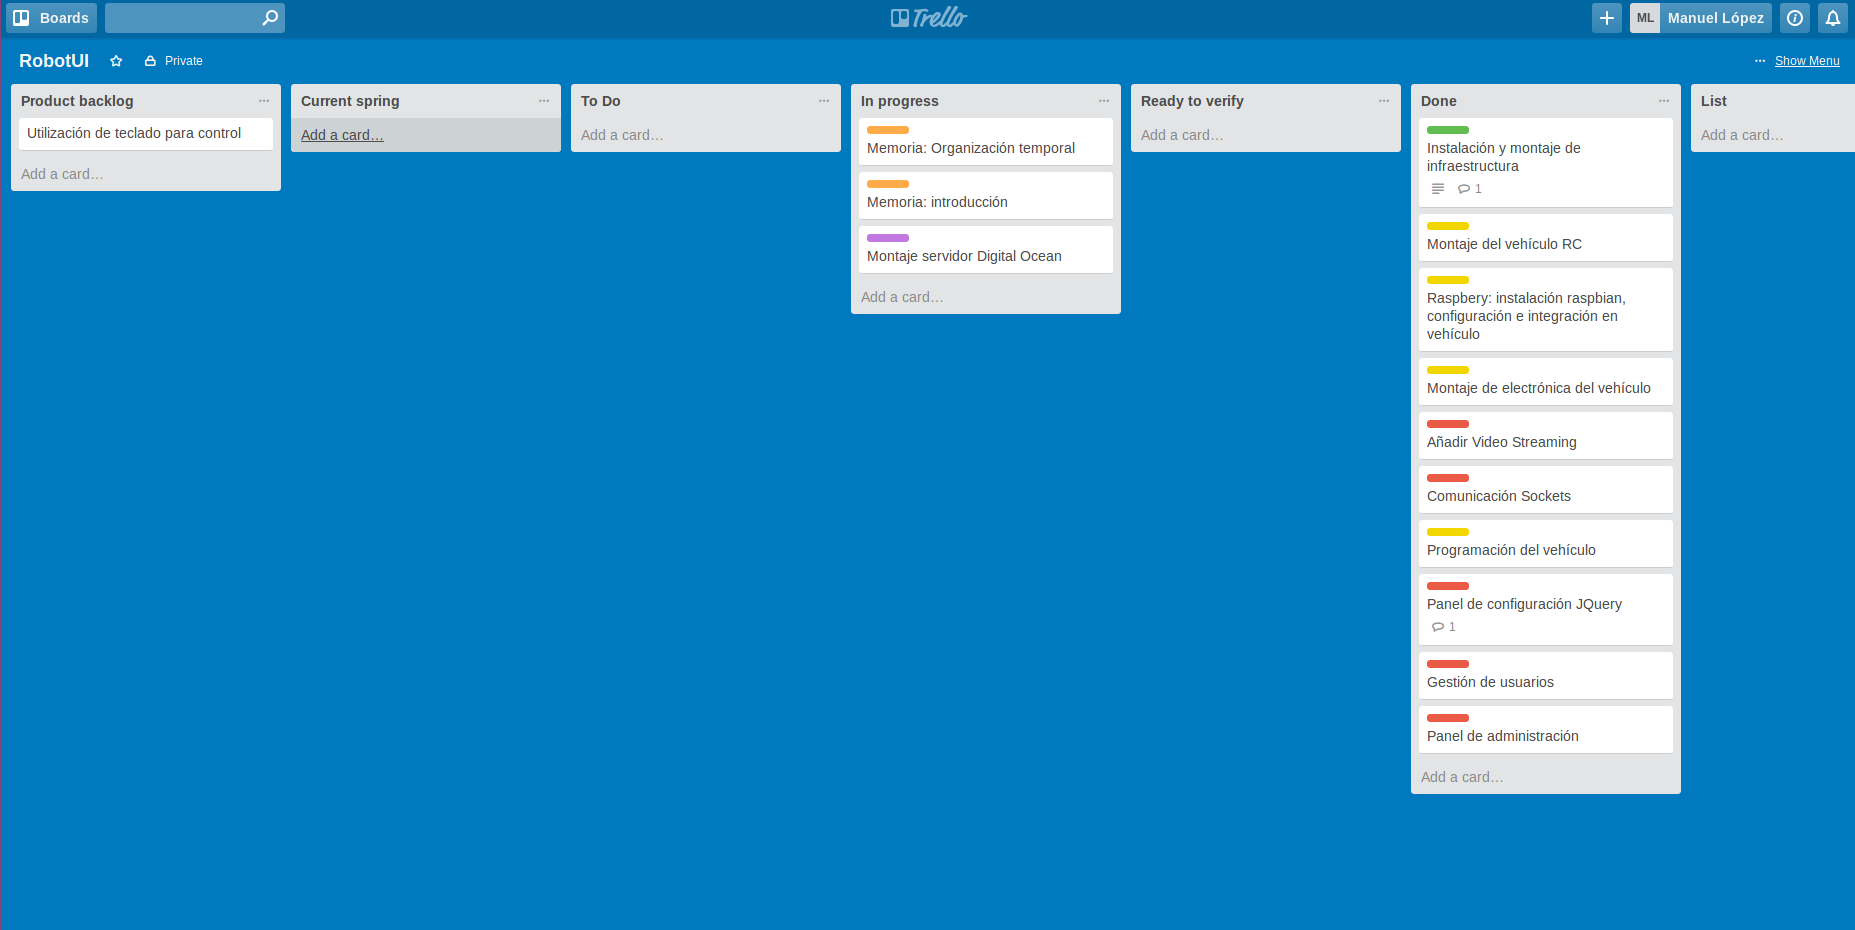
\includegraphics[scale=0.25]{imagenes/panel-trello.png}}
\caption{Panel de actividades - Trello}
\end{figure}

Los puntos más importantes del proyecto se han dividido en hitos, así como entregas que se definieron en cada reunión que se realizaba con el director del proyecto. También se ha definido una planificación temporal del desarrollo del proyecto mediante un diagrama de gantt con la duración de las tareas definidas en el panel de actividades de Trello.\\
\newpage


\section{Planificación temporal de tareas}

A continuación se definirán los diferentes hitos que componen el diagrama de Gantt así como las fechas estimadas para los cuales se realizaron los hitos:
\subsection{Hito 1: 1 Mayo a 1 Julio 2015}
\label{subsec:hito1}

En esta primera etapa de desarrollo del proyecto final de carrera, se realizaron los estudios de las tecnologías a implementar, la arquitectura del sistema, las tecnologías de BD, visualización, etc.

\subsection{Hito 2: 1 Julio a 1 Septiembre 2015}
\label{subsec:hito2}



\subsection{Hito 3: 1 Septiembre a 1 Noviembre 2015}
\label{subsec:hito3}


\subsection{Hito 4: 1 Noviembre 2015 a 1 Enero 2016}
\label{subsec:hito4}



\subsection{Hito 5: 1 Enero a 1 Marzo 2016}
\label{subsec:hito5}



\subsection{Hito 6: 1 Marzo a 1 Mayo 2016}
\label{subsec:hito6}


\section{Diagrama de Gantt}


